\thispagestyle{timhieukhoahocnone}
\pagestyle{timhieukhoahoc}
\everymath{\color{timhieukhoahoc}}
\blfootnote{$^1$\text{\color{timhieukhoahoc}Hà Nội.}}
\graphicspath{{../timhieukhoahoc/pic/}}
\begingroup
\AddToShipoutPicture*{\put(0,616){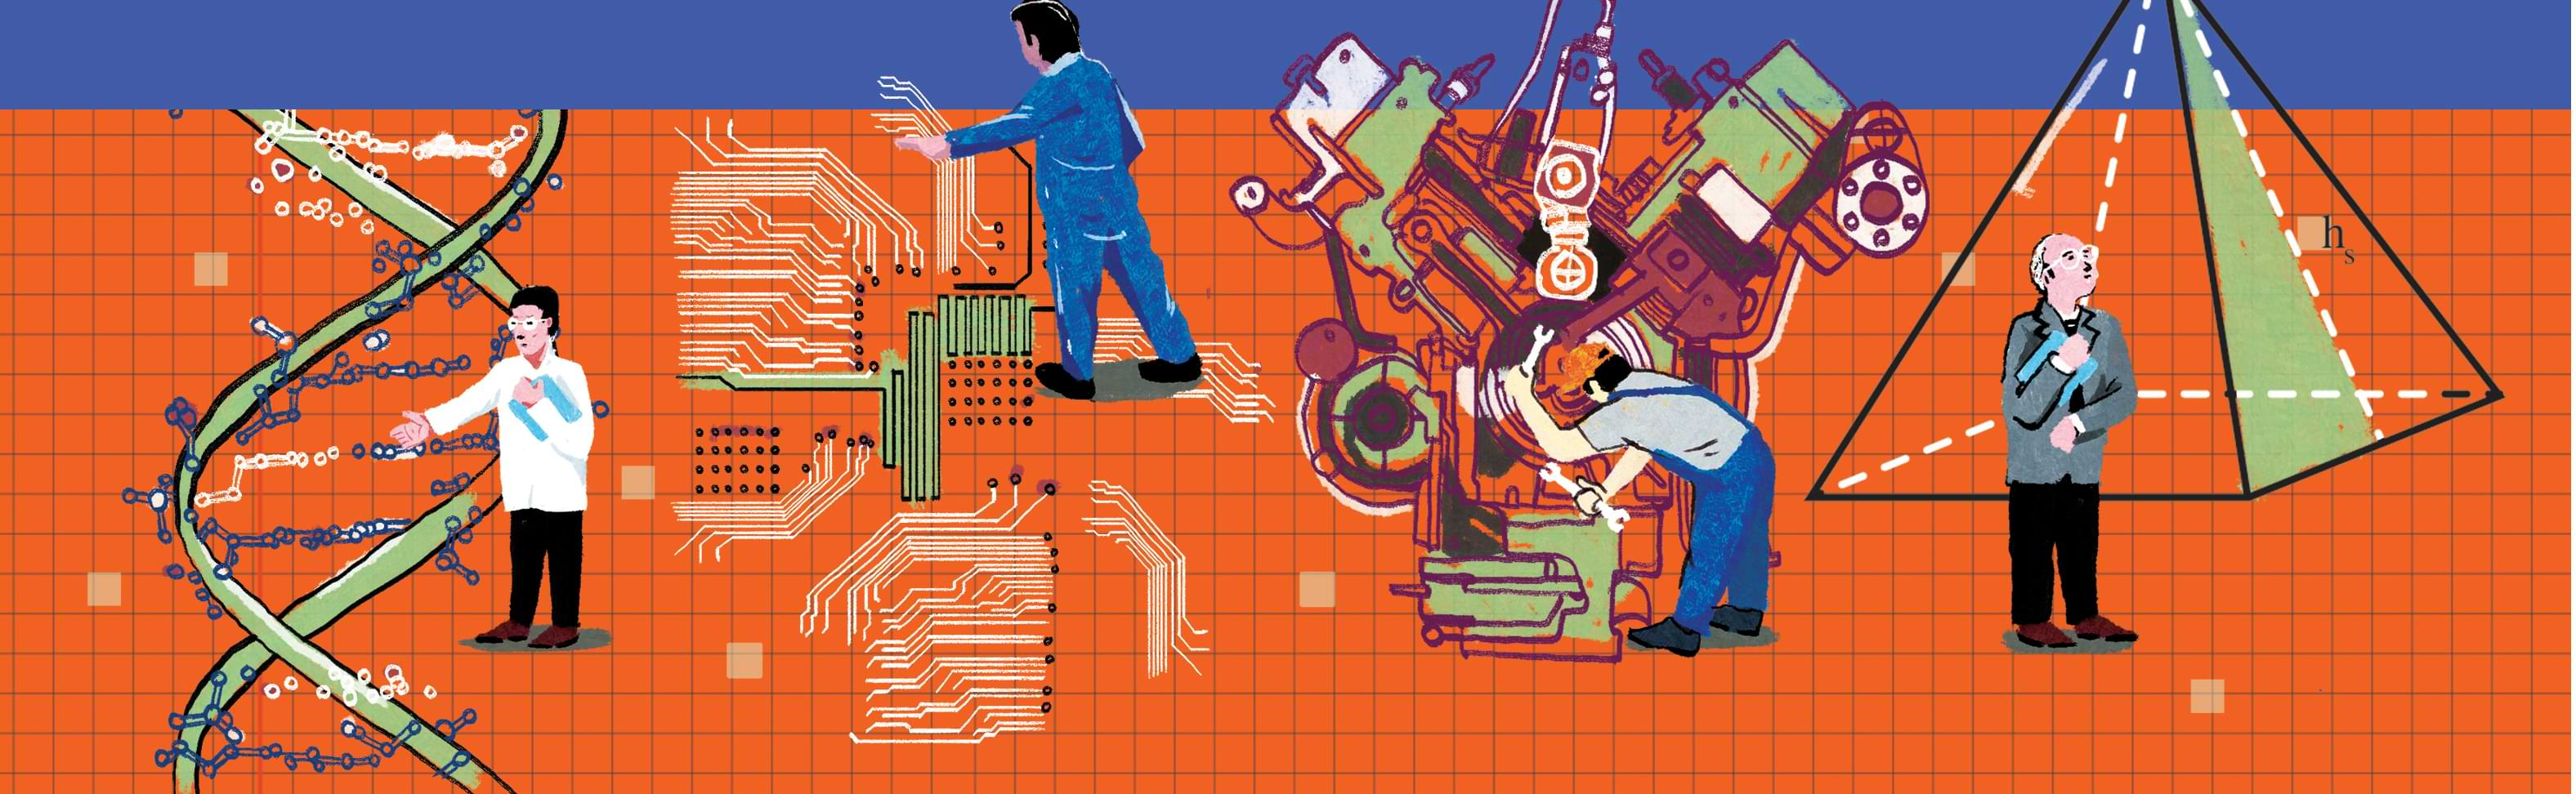
\includegraphics[width=19.3cm]{../bannertimhieu}}}
\AddToShipoutPicture*{\put(76,555){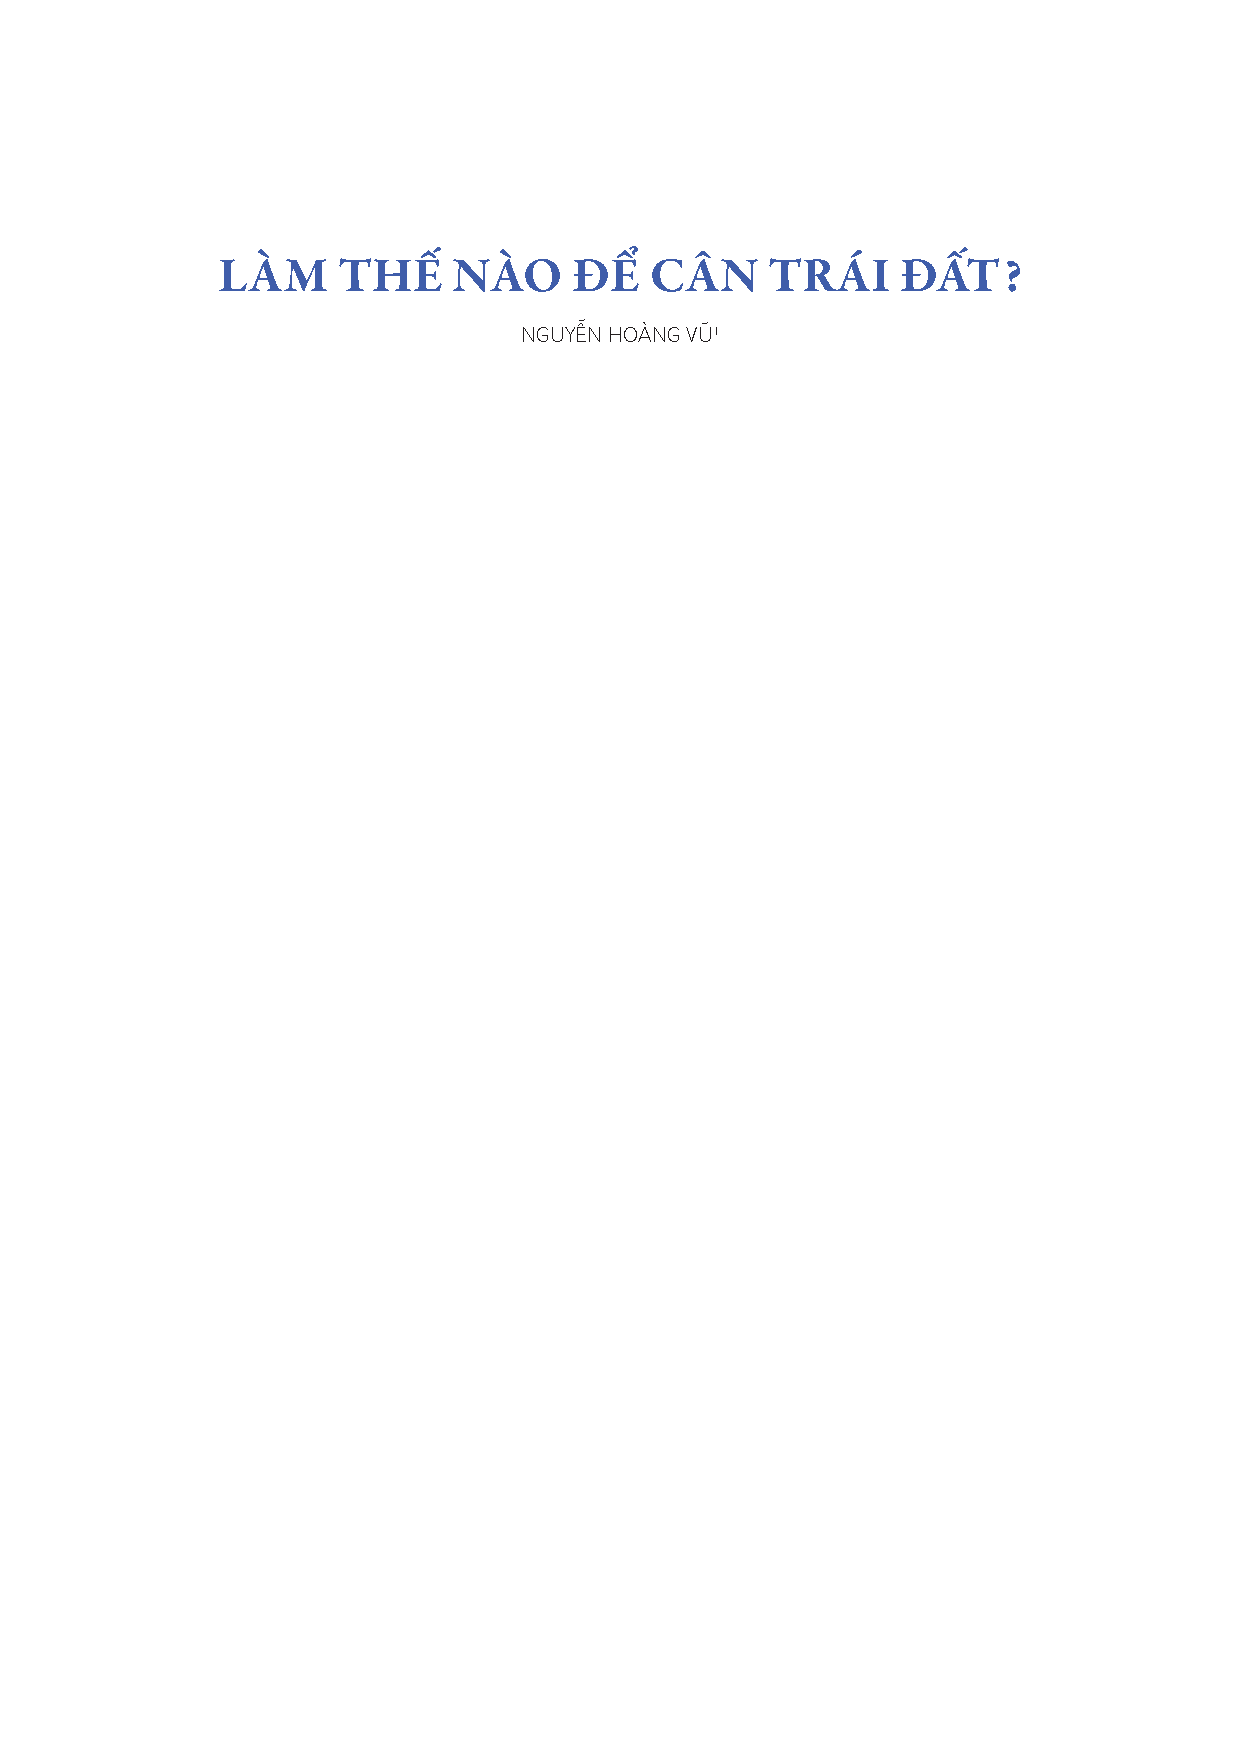
\includegraphics[scale=1]{../tieude.pdf}}}
\centering
\endgroup
\vspace*{155pt}

\begin{multicols}{2}
	Khối lượng của Trái Đất bằng bao nhiêu? Đây là một câu hỏi mà đến thế kỷ $18$ người ta mới có được những kết quả đo đạc tương đối chính xác dựa trên những lý thuyết vật lý được phát triển suốt hai thế kỷ bắt đầu từ những thí nghiệm của Galileo.
	\vskip 0.1cm
	$\pmb{1.}$ \textbf{\color{timhieukhoahoc}Từ Galileo đến Newton}
	\begin{figure}[H]
		\vspace*{-5pt}
		\centering
		\captionsetup{labelformat= empty, justification=centering}
		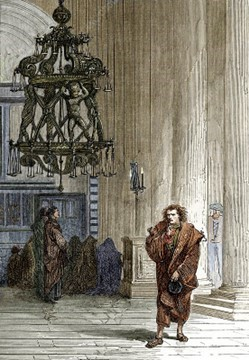
\includegraphics[width= 0.75\linewidth]{1}
		\caption{\small\textit{\color{timhieukhoahoc}Hình ${1.}$ Galileo và dao động của ngọn đèn trên trần nhà thờ.}}
		\vspace*{-10pt}
	\end{figure}
	Một câu chuyện khá thú vị thường được kể về Galileo và trọng lực là khi ông quan sát ngọn đèn trên trần nhà trong nhà thờ Pisa. Ông dùng mạch đập của mình để tính thời gian của mỗi chu kỳ dao động của nó và nhận thấy rằng với những góc dao động nhỏ, chu kỳ dao động không thay đổi. Với những thí nghiệm sau này về con lắc đơn, Galileo còn nhận thấy rằng chu kỳ dao động thay đổi theo chiều dài của dây treo (dây treo càng dài thì chu kỳ càng lớn) nhưng lại không phụ thuộc vào khối lượng của con lắc.
	\begin{figure}[H]
		\vspace*{-5pt}
		\centering
		\captionsetup{labelformat= empty, justification=centering}
		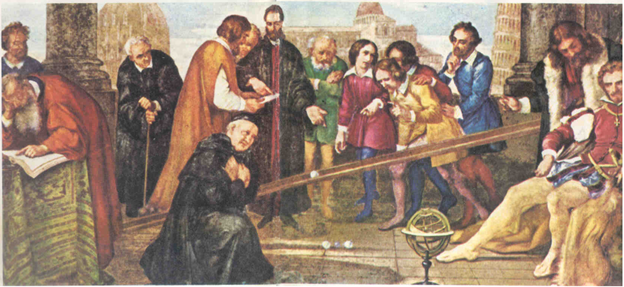
\includegraphics[width= 1\linewidth]{2}
		\caption{\small\textit{\color{timhieukhoahoc}Hình $2$. Galileo biểu diễn thí nghiệm về chuyển động trên mặt phẳng nghiêng cho các quý tộc nhà Medici (tranh của Giuseppe  Bezzuoli).}}
		\vspace*{-10pt}
	\end{figure}
	Ông tiếp tục nghiên cứu vấn đề này bằng cách làm thí nghiệm với chuyển động trên mặt phẳng nghiêng, một dạng chuyển động mà ông cho rằng có thể dùng để liên hệ với chuyển động theo cung tròn của con lắc. Thời gian được Galileo đo bằng một đồng hồ nước. Khi hòn bi được thả từ vị trí đầu của mặt phẳng nghiêng thì khóa cũng được mở để nước từ đồng hồ chảy vào một bình chứa bên dưới. Khi hòn bi đến vị trí bị chặn lại thì khóa cũng được đóng lại cùng lúc. Việc đo lượng nước trong bình sẽ cho độ dài thời gian của chuyển động. Kết quả thí nghiệm cho thấy quãng đường chuyển động tỷ lệ thuận với bình phương của thời gian. Đồng thời, thời gian chuyển động cho cùng một quãng đường sẽ càng ngắn khi góc nghiêng tăng lên.
	\vskip 0.1cm
	Galileo còn phát hiện ra rằng khi cho hòn bi lăn trên một dây cung có điểm cuối tại vị trí mà đường tròn tiếp xúc phương nằm ngang thì thời gian chuyển động không thay đổi khi ta di chuyển vị trí đầu dây cung trên đường tròn (độc giả có thể thử tự chứng minh bài toán này). Đồng thời, ta cũng có thể coi chuyển động của con lắc đơn dọc theo cung tròn là tổng hợp của nhiều chuyển động trên các đoạn dây cung liên tiếp nhau. Nhận định này cũng là cơ sở giúp Huygens thiết lập phương trình toán học cho chuyển động của con lắc đơn nhiều thập kỷ sau đó.
	\begin{figure}[H]
		\vspace*{-5pt}
		\centering
		\captionsetup{labelformat= empty, justification=centering}
		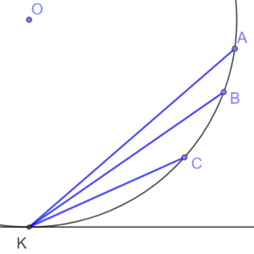
\includegraphics[height= 0.45\linewidth]{3a}
		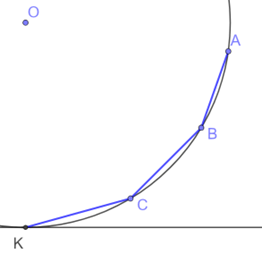
\includegraphics[height= 0.45\linewidth]{3b}
		\caption{\small\textit{\color{timhieukhoahoc}Hình $3.$ Một số nhận định của Galileo về chuyển động trên mặt phẳng nghiêng. Trái: viên bi lăn trên các dây cung của cùng một đường tròn và cùng một điểm cuối có thời gian lăn bằng nhau. Phải: Khi xấp xỉ cung tròn bằng các đoạn mặt phẳng nghiêng liên tiếp, thời gian lăn càng ngày càng gần với thời gian lăn trên cung tròn khi độ dài các đoạn nghiêng càng nhỏ.}}
		\vspace*{-10pt}
	\end{figure}
	Một điểm đáng chú ý nữa là khi dây cung trở thành đường kính, ta có được chuyển động rơi tự do! Khi đó, quãng đường chuyển động của vật rơi tự do sẽ tỷ lệ với bình phương thời gian. Mặt khác, độ dài của dây treo con lắc đơn cũng tỷ lệ với bình phương của chu kỳ dao động. Galileo tiến hành các thí nghiệm đo tỷ lệ giữa thời gian rơi tự do và chu kỳ con lắc đơn, với độ cao thả rơi bằng chiều dài dây treo của con lắc. Kết quả cho thấy đây là một hằng số không phụ thuộc vào khối lượng. Các thí nghiệm của ông cho kết quả từ $2{,}3$ đến $2{,}52$ (giá trị đúng là $\dfrac{g}{\sqrt{2}}=2{,}22$). Do không có cơ sở lý thuyết, Galileo không thể đưa ra chứng minh toán học cho vấn đề này.
	\vskip 0.1cm
	Quy luật bình phương thời gian của chuyển động trong các thí nghiệm của Galileo hoàn toàn đi ngược lại với những lập luận của Aristotle. Trong khi Aristotle phát biểu rằng vật càng nặng sẽ rơi càng nhanh hơn, Galileo lại kết luận bằng thực nghiệm rằng thời gian rơi chỉ phụ thuộc vào độ cao khi thả vật. Việc thay những lập luận cảm tính bằng kiểm chứng thực nghiệm đánh dấu một chuyển biến lớn, đặt nền móng cho khoa học tự nhiên hiện đại.
	\begin{figure}[H]
		\vspace*{-5pt}
		\centering
		\captionsetup{labelformat= empty, justification=centering}
		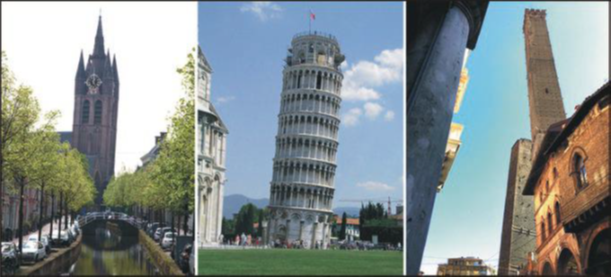
\includegraphics[width =1\linewidth]{4}
		\caption{\small\textit{\color{timhieukhoahoc}Hình $4$. Các ngọn tháp nghiêng gắn liền với các thí nghiệm về trọng lực. Trái: Tháp nghiêng Oude Kerk (Hà Lan). Giữa: Tháp nghiêng Pisa (Italia). Phải: Tháp nghiêng Asinelli (Italia).}}
		\vspace*{-10pt}
	\end{figure}
	Nhiều độc giả chắc cũng sẽ liên hệ đến câu chuyện về Galileo và tháp nghiêng Pisa, trong đó khi ông thả cùng lúc một quả đạn đại bác và một viên đạn súng trường từ đỉnh tháp thì chúng cũng chạm đất cùng một thời điểm. Tuy nhiên, về mặt lịch sử, Galileo không phải là người đầu tiên làm việc này. Một thí nghiệm tương tự đã được Simon Stevin tiến hành trước đó vào năm $1586$ tại tháp nghiêng ở Oude Kerk (Delft, Hà Lan). Sau vài thập kỷ, một thí nghiệm quan trọng hơn được Giovanni Riccioli thực hiện tại tháp nghiêng Asinelli ở Bologna, Italia bắt đầu từ năm $1640$. Thời gian rơi từ các độ cao khác nhau cho kết quả hoàn toàn khớp với quy luật bình phương thời gian. Những số liệu của Riccioli cho thấy giá trị gia tốc trọng trường là $9{,}4 \,m/s^2$, không quá xa so với giá trị đã biết ngày nay. 
	\vskip 0.1cm
	Mặt khác, vào đầu thế kỷ $17$, dựa vào những số liệu thiên văn của Tycho Brahe, Kepler đã đưa ra các định luật quan trọng về sự chuyển động của các hành tinh quanh Mặt Trời. Quỹ đạo của các hành tinh là một hình ellipse mà Mặt Trời nằm tại một tiêu điểm của nó. Tuy nhiên, Kepler vẫn chưa đưa ra được giải thích đầy đủ cho hiện tượng này. Phải vài thập kỷ tiếp theo, lý thuyết về lực hấp dẫn mới được hình thành trong các nghiên cứu của Newton. Một điều đáng chú ý là Newton không phải người đầu tiên đưa ra giả thuyết về một lực hấp dẫn tỷ lệ nghịch với bình phương khoảng cách. Nhà toán học Pháp Ismael Boulliau đã thảo luận về vấn đề này năm $1645$, nhưng Newton chính là người đầu tiên đưa ra được chứng minh toán học rằng một lực như vậy sẽ dẫn đến các quỹ đạo ellipse như trong định luật $1$ của Kepler, cũng như các quỹ đạo dạng conic khác (tròn, parabol và hyperbol). Đồng thời, Newton cũng tính toán được rằng lực hấp dẫn của một khối cầu đối với một vật khác sẽ tương đương với lực hấp dẫn của chất điểm có cùng khối lượng đặt ở tâm hình cầu. Nói cách khác, trọng lực gây ra sự rơi của các vật hướng về mặt đất cũng như lực hút giữa các vật thể trong vũ trụ có cùng bản chất.
	\vskip 0.1cm
	Lực hấp dẫn giữa hai vật có khối lượng $m_1$ và $m_2$ cách nhau một khoảng $r$ có công thức như sau:
%	\setlength{\abovedisplayskip}{5pt}
%	\setlength{\belowdisplayskip}{5pt}
	\begin{align*}
		F =\frac{Gm_1m_2}{r^2}
	\end{align*}
	với $G$ là hằng số hấp dẫn. Cần chú ý rằng khái niệm về $G$ chưa xuất hiện ở thời kỳ của Newton.
	\vskip 0.1cm
	$\pmb{2.}$ \textbf{\color{timhieukhoahoc}Lực hấp dẫn của ngọn núi}
	\vskip 0.1cm
	Một vấn đề được đặt ra là trọng lực liệu có như nhau tại mọi nơi trên Trái Đất? Theo Newton, do lực quán tính ly tâm, Trái Đất sẽ phình ra hơn ở xích đạo và do đó trọng lực sẽ nhỏ nhất ở vị trí này và tăng dần theo vĩ độ. Từ các kết quả đo đạc trọng lực của nhà khoa học Pháp Jean Richer tại đảo Cayenne, Newton tính ra rằng khoảng cách đến tâm Trái Đất tại xích đạo lớn hơn tại các cực là $17$ dặm (con số chính xác là $13$ dặm).
	\vskip 0.1cm
	Tuy nhiên, tại bản thân nước Pháp, nhiều nhà khoa học ủng hộ lý thuyết của Descartes từ hơn nửa thế kỷ trước, rằng tương tác giữa các vật thể trong vũ trụ hay trọng lực đều xảy ra do các vòng xoáy của một chất lỏng vô hình tràn đầy khắp nơi gọi là ``ether", ngược với mô hình lực hấp dẫn của Newton. Một số đo đạc tại Pháp của hai cha con Cassini, đều là thành viên Viện Hàn lâm Khoa học Pháp, vào đầu thế kỷ $18$ cho kết quả rằng độ dài của vĩ độ giảm dần khi vĩ độ tăng, tức Trái Đất nhọn ở hai cực (dạng quả trứng). Trong khi đó, những người Anh lại cho rằng các đo đạc tại Pháp có độ chính xác không đủ cao.
	\begin{figure}[H]
		\vspace*{-6pt}
		\centering
		\captionsetup{labelformat= empty, justification=centering}
		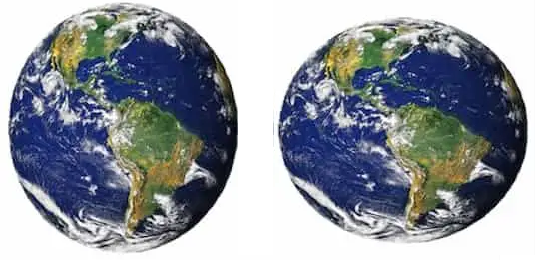
\includegraphics[width =1\linewidth]{5}
		\caption{\small\textit{\color{timhieukhoahoc}Hình $5$. Trái Đất dẹt ở xích đạo hay ở hai cực? Đây là một câu hỏi quan trọng của khoa học thế kỷ $18$.}}
		\vspace*{-10pt}
	\end{figure}
	Năm $1734$, Johann Bernoulli công bố chứng minh của ông rằng các xoáy ether của Descartes sẽ dẫn đến việc Trái Đất nhọn ở hai đầu, cung cấp cơ sở lý thuyết cho thuyết quả trứng. Trong khi đó, học trò của ông là Pierre Maupertuis lại ủng hộ mô hình của Newton. Bản thân Viện Hàn lâm Khoa học Pháp bị chia thành hai phái do vấn đề này.
	\vskip 0.1cm
	Sau khi Pháp và Tây Ban Nha trở thành đồng minh, năm $1735$, một đoàn khảo sát gồm ba thành viên của Viện Hàn lâm Khoa học Pháp: Pierre Bouger, Charles--Marie de La Condamine và Louis Godin được cử đến khu vực dãy núi Andes ở Nam Mỹ do Tây Ban Nha quản lý lúc đó để tiến hành đo độ dài của vĩ độ ở xích đạo. Đồng thời, năm $1736$, Maupertuis đích thân dẫn đoàn đi đo độ dài vĩ độ tại Lapland, Phần Lan. Các kết quả của hai chuyến khảo sát này cho thấy Newton đã đúng: Trái Đất phình ra hơn ở xích đạo và dẹt hơn ở hai cực.
	\begin{figure}[H]
		\vspace*{-5pt}
		\centering
		\captionsetup{labelformat= empty, justification=centering}
		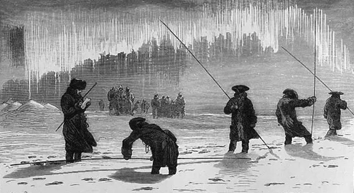
\includegraphics[width =1\linewidth]{6}
		\caption{\small\textit{\color{timhieukhoahoc}Hình $6$. Maupertuis đo độ dài vĩ độ tại Lapland.}}
		\vspace*{-10pt}
	\end{figure}
	Trong thời gian này, Bouger cũng đã tiến hành đo trọng lực tại những độ cao và vĩ độ khác nhau thông qua việc xác định chu kỳ của con lắc đơn. Bouger đã chỉ ra ba nhân tố ảnh hưởng đến giá trị của gia tốc trọng trường $g$ trong thực tiễn:
	\vskip 0.1cm
	$\bullet$ Vĩ độ: khi vĩ độ tăng, khoảng cách từ vị trí của ta đến trục quay của Trái Đất cũng tăng nên lực quán tính ly tâm do chuyển động quay của Trái Đất cũng giảm theo.
	\vskip 0.1cm
	$\bullet$ Độ cao: Tại độ cao $h$ so với mực nước biển, ta có $g = \dfrac{GM}{(R +h)^2}$ với $G$ là hằng số hấp dẫn, còn $M$ và $R$ lần lượt là khối lượng và bán kính Trái Đất. Sử dụng xấp xỉ bậc nhất ta có: $g \approx \dfrac{GM}{R^2}\left(1 - \dfrac{2h}{R}\right)$.
	\vskip 0.1cm
	$\bullet$ Địa hình: Do khoảng không giữa vị trí đo và mực nước biển không phải là không khí mà là dãy núi, Bouger tiến hành tính toán ảnh hưởng từ lực hấp dẫn của các đối tượng này lên giá trị trọng lực đo được. Nếu coi toàn bộ khoảng không giữa Trái Đất (bán kính $R$) và vị trí đo có một vỏ cầu bề dày $h$ thì thành phần trọng lực do vỏ cầu này gây ra tại độ cao $h$ sẽ bằng $4\pi Gh\rho'$ với $\rho'$ là mật độ của vỏ cầu. Để mô phỏng tốt hơn dãy núi Andes, Bouger sử dụng một hình lăng trụ dài vô hạn có thiết diện là một tam giác vuông cân. Từ trường hợp này, có thể tính được thành phần trọng lực với các giá trị khác nhau của góc giữa hai cạnh bên của dãy núi. Khi hai cạnh của dãy núi tạo với nhau góc $180^\circ$, ta được mặt phẳng Bouger, một mặt phẳng giả tưởng mà ngay nay vẫn được các nhà địa vật lý sử dụng để hiệu chỉnh giá trị đo trọng lực.
	\begin{figure}[H]
		\vspace*{-5pt}
		\centering
		\captionsetup{labelformat= empty, justification=centering}
		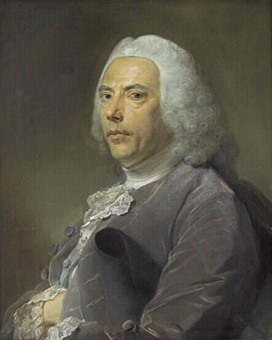
\includegraphics[width =0.75\linewidth]{7}
		\caption{\small\textit{\color{timhieukhoahoc}Pierre Bouger $(1698 - 1758)$.}}
		\vspace*{-10pt}
	\end{figure}
	Từ dữ liệu ở hai điểm có độ cao khác nhau, Bouger tính được rằng tỷ lệ mật độ của dãy núi Andes so với mật độ của Trái Đất là $\dfrac{850}{3993}$. Giá trị mật độ đo được ngày nay của dãy Andes và Trái Đất lần lượt là $2{,}7$ và $5{,}515\, g/cc$. Tuy giá trị mà Bouger tính được không chính xác nhưng nó cho thấy một phương pháp để xác định khối lượng Trái Đất (khi đã biết bán kính của nó): đánh giá biến thiên trọng lực gây ra bởi một ngọn núi để tìm mật độ của Trái Đất.
	\vskip 0.1cm
	Để tiến hành tính khối lượng Trái Đất, Bouger và La Condamine cần một ngọn núi cách biệt với các ngọn núi khác (thay vì nhiều đỉnh núi liền nhau như Bouger đã đo trên dãy Andes) để việc ước lượng khối lượng của nó dễ dàng hơn. Họ chọn ngọn núi Chimborazo (ngày nay thuộc Ecuador).
	\begin{figure}[H]
		\vspace*{5pt}
		\centering
		\captionsetup{labelformat= empty, justification=centering}
		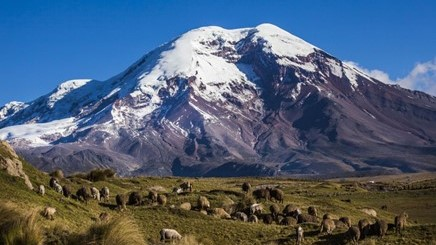
\includegraphics[width =1\linewidth]{8}
		\caption{\small\textit{\color{timhieukhoahoc}Hình $7$. Núi Chimborazo (Ecuador ngày nay).}}
		\vspace*{-10pt}
	\end{figure}
	Việc đo đạc được tiến hành năm $1738$ tại hai vị trí cùng vĩ độ: một ở xa và một ở gần ngọn núi (thay vì trên đỉnh núi). Khi đó ở vị trí gần ngọn núi, lực hấp dẫn của ngọn núi sẽ làm con lắc bị lệch khỏi phương thẳng đứng. Độ lệch này sẽ được xác định bằng cách so phương dây dọi với phương quan sát tới cùng một ngôi sao tại hai địa điểm. Sau khi xác định góc lệch do lực hấp dẫn của ngọn núi gây ra, tỷ lệ mật độ giữa ngọn núi và Trái Đất có thể được xác định thông qua biến đổi toán học (thể tích của ngọn núi cần được tính thông qua các công thức giải tích). Ước lượng cho khối lượng Trái Đất mà Bouger công bố sau khi trở lại Pháp không quá chính xác do những sai sót trong việc tính thể tích ngọn núi cũng như giả thuyết rằng lực hấp dẫn của ngọn núi tương đương với lực hấp dẫn của một chất điểm có cùng khối lượng đặt ở trọng tâm (giả thuyết này chỉ đúng với hình cầu).
	\begin{figure}[H]
		\vspace*{-5pt}
		\centering
		\captionsetup{labelformat= empty, justification=centering}
		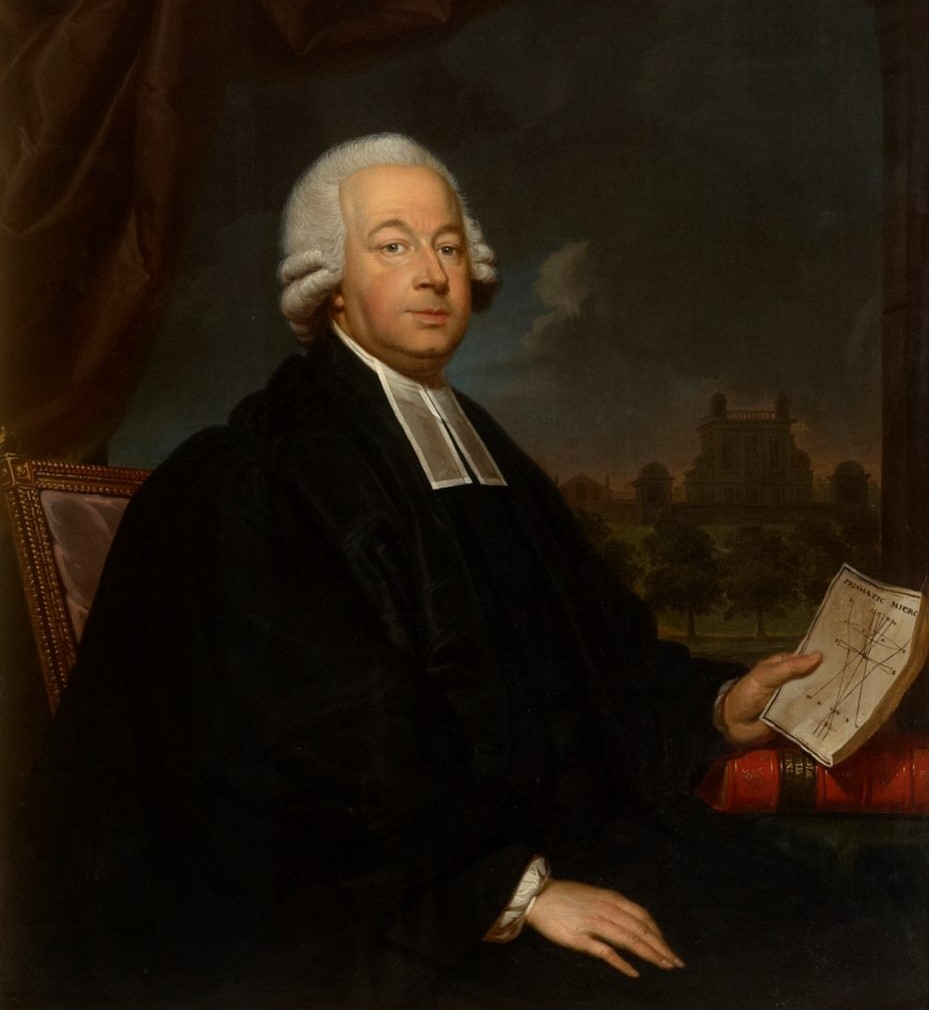
\includegraphics[width =0.75\linewidth]{9}
		\caption{\small\textit{\color{timhieukhoahoc}Nevil Maskelyne $(1732-1811)$.}}
		\vspace*{-5pt}
	\end{figure}
	Dù Bouger đề nghị các nhà khoa học khác ở châu Âu tiến hành những thí nghiệm tương tự, phải nhiều năm sau việc này mới lại được nhắc đến. Năm $1772$, Nevil Maskelyne đề xuất tiến hành một thí nghiệm như vậy tại Anh. Cuối cùng, ngọn núi Schiehallion ở Scotland được chọn do nó đủ lớn, cách xa các đỉnh núi khác và có hình dạng dễ tính toán. Các dữ liệu từ lần đo này được nhà toán học Charles Hutton xử lý. Kết quả cuối cùng cho mật độ Trái Đất là $4{,}5 \,g/cc$. Nếu sử dụng các dữ liệu hiện đại về địa hình cũng như mật độ của đá núi tại địa điểm đó, kết quả đúng sẽ là $5{,}480\, g/cc$, rất gần với giá trị $5{,}515\, g/cc$ ngày nay.
	\begin{figure}[H]
		\vspace*{-5pt}
		\centering
		\captionsetup{labelformat= empty, justification=centering}
		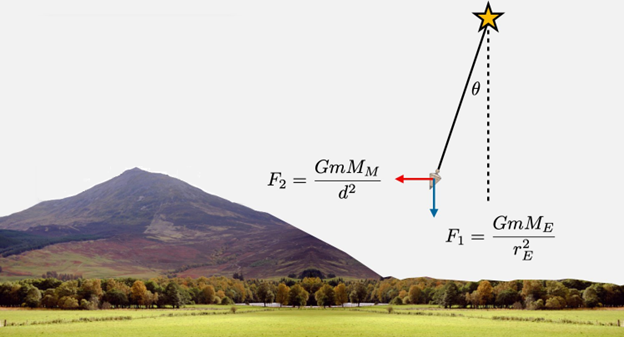
\includegraphics[width =1\linewidth]{10}
		\caption{\small\textit{\color{timhieukhoahoc}Hình $8$. Thí nghiệm ở  núi Schiehallion (Scotland).}}
		\vspace*{-10pt}
	\end{figure}
	Một điểm đáng chú ý là Hutton đã biểu diễn các điểm có cùng độ cao bằng một đường gấp khúc khi mô tả địa hình của khu vực xung quanh Schiehallion. Các đường này đã trở thành các đường đồng mức được sử dụng phổ biến trong bản đồ địa hình cũng như trong các biểu diễn dữ liệu kỹ thuật. 
	\begin{figure}[H]
		\vspace*{-5pt}
		\centering
		\captionsetup{labelformat= empty, justification=centering}
		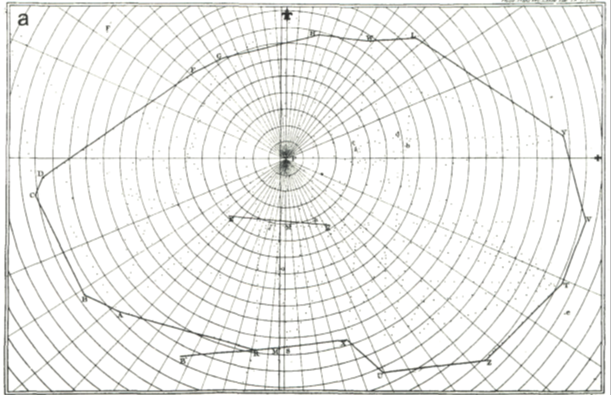
\includegraphics[width =1\linewidth]{11}
		\caption{\small\textit{\color{timhieukhoahoc}Hình $9$. Đường đồng mức độ cao của Charles Hutton.}}
		\vspace*{-5pt}
	\end{figure}
	\vspace*{1pt}
	
	\vspace*{-8pt}
	\PIbox{Trong thế kỷ $19$, với các cuộc khảo sát sử dụng con lắc đơn để đo trọng lực ở khu vực Ấn Độ, các nhà khoa học Anh đã nhận thấy độ lệch của con lắc khi ở gần dãy núi Himalaya không lớn như các tính toán lý thuyết. Các nghiên cứu của các nhà khoa học John Pratt và George Airy về vấn đề này đã dẫn đến mô hình trong đó lớp vỏ Trái Đất thực chất đang nổi trên một lớp dung nham nóng chảy ở phía dưới. Phải đến giữa thế kỷ $20$, người ta mới khẳng định được vấn đề này nhờ các phát hiện chứng minh cho thuyết kiến tạo lục địa.}
	\vskip 0.2cm
	$\pmb{3.}$ \textbf{\color{timhieukhoahoc}Thí nghiệm của Cavendish}
	\vskip 0.1cm
	Liệu có cách nào để đo khối lượng Trái Đất mà không cần đi đến những ngọn núi xa xôi? Năm $1797$, Henry Cavendish đã tiến hành một thí nghiệm như vậy ngay tại London. Dựa trên những thiết bị chưa hoàn thiện của John Michell, ông đã thiết kế thí nghiệm đo lực hấp dẫn thông qua momen xoắn.
	\begin{figure}[H]
		\vspace*{-5pt}
		\centering
		\captionsetup{labelformat= empty, justification=centering}
		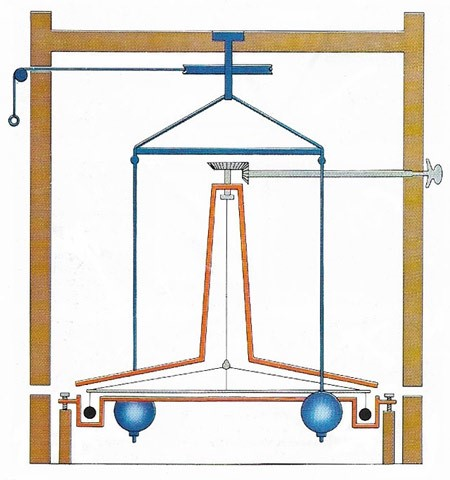
\includegraphics[width =1\linewidth]{12}
		\caption{\small\textit{\color{timhieukhoahoc}Hình $10$. Sơ đồ thí nghiệm của Cavendish. Các viên bi m có màu đen còn các quả nặng bằng chì $M$ có màu xanh.}}
		\vspace*{-10pt}
	\end{figure}
	Về cơ bản, ta có hai quả cầu nhỏ $m$ và hai quả cầu lớn $M$ bằng chì. Lực hấp dẫn do các quả cầu lớn tác dụng lên các quả cầu nhỏ sẽ tạo một momen xoắn làm xoay dây treo. Bằng cách xác định góc lệch của thanh nối hai quả cầu nhỏ, ta có thể tính được momen xoắn cũng như độ lớn của lực hấp dẫn.
	\begin{figure}[H]
		\vspace*{-5pt}
		\centering
		\captionsetup{labelformat= empty, justification=centering}
		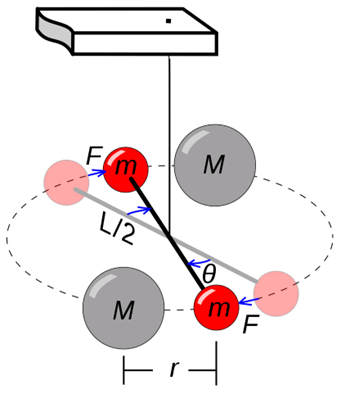
\includegraphics[width =1\linewidth]{13}
		\caption{\small\textit{\color{timhieukhoahoc}Hình $11$. Các lực hấp dẫn tạo momen xoắn làm lệch dây treo.}}
		\vspace*{-10pt}
	\end{figure}
	Do khoảng cách giữa $M$ với $m$ và khoảng cách từ $m$ đến tâm Trái Đất cũng như khối lượng của $m$ đều là đã biết, thí nghiệm của Cavendish cho phép xác định khối lượng Trái Đất qua tỷ lệ giữa lực hút của $M$ với $m$ và trọng lực tác dụng lên $m$. Với giả sử Trái Đất là hình cầu, kết quả của Cavendish cho mật độ của Trái Đất là $5{,}448 g/cc$.
	\vskip 0.1cm
	Bản thân thí nghiệm này cũng cho phép tính được hằng số hấp dẫn $G$ từ độ lớn của lực hấp dẫn giữa $M$ và $m$. Số liệu của Cavendish cho giá trị của $G$ chỉ khác $1\%$ so với số liệu hiện đại nhất. Cho đến ngày nay, việc đo momen xoắn vẫn là phương pháp chủ yếu cho các thí nghiệm độ chính xác cao để xác định hằng số hấp dẫn.
	\vskip 0.1cm
	$\pmb{4.}$ \textbf{\color{timhieukhoahoc}Đo trọng lực thời hiện đại}
	\vskip 0.1cm
	Trong thế kỷ $19$, đã có một số nỗ lực cải thiện độ chính xác của việc đo trọng lực. Vào đầu thế kỷ, Henry Kater đề xuất sử dụng con lắc vật lý thay cho con lắc đơn. Con lắc này gồm một vật nặng cố định $W_2$ và một vật nặng có thể di chuyển $W_1$. Trọng tâm $G$ của hệ sẽ thay đổi khi $W_1$ di chuyển. Con lắc Kater có thể được cho dao động quanh một trong hai điểm tựa $O_1$ hoặc $O_2$. Gọi $h_1$ và $h_2$ là khoảng cách từ các điểm này đến $G$.
	\begin{figure}[H]
		\vspace*{-5pt}
		\centering
		\captionsetup{labelformat= empty, justification=centering}
		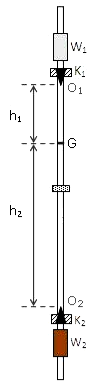
\includegraphics[width =0.3\linewidth]{14}
		\caption{\small\textit{\color{timhieukhoahoc}Hình $12.$ Con lắc thuận nghịch của Kater.}}
		\vspace*{-10pt}
	\end{figure}
	Khi dao động quanh $O_1$, momen quán tính của con lắc là $I_1=I_G+Mh_1^2$ với $I_G$ là momen quán tính của con lắc quanh $G$ và $M$ là tổng khối lượng của cả hệ. Phương trình dao động cho góc lệch nhỏ khi đó là:
	\begin{align*}
		I_1\theta''=-Mgh_1 \theta
	\end{align*}
	cho ta chu kỳ dao động:
	\begin{align*}
		T_1 = 2\pi \sqrt{\frac{\left(h_1^2 + \frac{I_G}{M}\right)}{gh_1}}
	\end{align*}
	Tương tự cho $T_2$, sau khi biến đổi đại số ta có:
	\begin{align*}
		h_1T_1^2 - h_2T_2^2 = \frac{4 \pi^2}{g}\left(h_1^2 - h_2^2\right)
	\end{align*}
	do đó:
	\begin{align*}
		g = \frac{8\pi^2}{\dfrac{T_1^2 + T_2^2}{h_1 + h_2} + \dfrac{T_1^2 -T_2^2}{h_1 - h_2}}.
	\end{align*}
	Khi $h_1=h_2$, ta có $T_1=T_2=T$ và $g=\dfrac{4\pi^2}{T^2}(h_1+h_2)$.
	\vskip 0.1cm
	Khi sử dụng, người ta cần chỉnh vị trí của $W_1$ sao cho $T_1=T_2$ trong khi đó $h_1+h_2$ chính là khoảng cách $O_1O_2$ đã biết.
	\vskip 0.1cm
	Thiết kế này được nhà toán học Friedrich Bessel cải tiến bằng cách cho khối lượng của $W_1$ và $W_2 $bằng nhau. Khi đó, với các giá trị của $T_1$ và $T_2$ gần nhau, có thể tính được T theo công thức:
	\begin{align*}
		T^2 = \frac{T_1^2 + T_2^2}{2} + \frac{T_1^2 - T_2^2}{2}\left(\frac{h_1 + h_2}{h_1 - h_2}\right).
	\end{align*}
	Với thay đổi này, việc hiệu chỉnh con lắc trở nên đỡ phức tạp hơn nhiều.
	\vskip 0.1cm
	Đến cuối thế kỷ $19$, nhà vật lý Eötvös bắt đầu sử dụng các thiết bị tương tự như của Cavendish để đo trọng lực phục vụ khảo sát địa chất ở Hungary. Một số thiết bị dạng này cũng được sản xuất ở một số nơi khác nhau trên thế giới. Người ta hi vọng rằng việc khảo sát sự biến thiên của trọng lực ở các vị trí khác nhau có thể giúp phát hiện các bất thường dưới lòng đất như mỏ quặng, mỏ dầu, khí gas, ... Tuy nhiên, việc đo đạc chiếm thời gian quá dài và đòi hỏi độ chính xác cao khi thao tác là một khó khăn lớn.
	\vskip 0.1cm
	Đến giai đoạn trước chiến tranh thế giới thứ hai, Lucien LaCoste, khi đang theo học cao học tại đại học Texas, Austin, đã phát minh ra một thiết bị đo trọng lực mới sử dụng lò xo. Ý tưởng về việc sử dụng lực đàn hồi lò xo để đo trọng lực đã được đưa ra từ thế kỷ $19$ nhưng nhiều vấn đề về kỹ thuật đã dẫn đến việc thiết kế thiết bị dạng này không hiệu quả. LaCoste sử dụng một loại lò xo ``độ dài zero". Với loại lò xo này, sẽ có một khoảng hoạt động mà trong đó lực đàn hồi tỷ lệ thuận với độ dài lò xo (thay vì tỷ lệ thuận với độ lệch từ độ dài tự nhiên). Các trọng lực kế theo dạng LaCoste có độ chính xác cao và nhanh chóng được sử dụng phổ biến ngày nay trong các khảo sát địa chất. Trọng lực kế của công ty LaCoste còn được NASA đưa lên Mặt Trăng để khảo sát trọng lực trên thiên thể này.
	\begin{figure}[H]
		\vspace*{-5pt}
		\centering
		\captionsetup{labelformat= empty, justification=centering}
		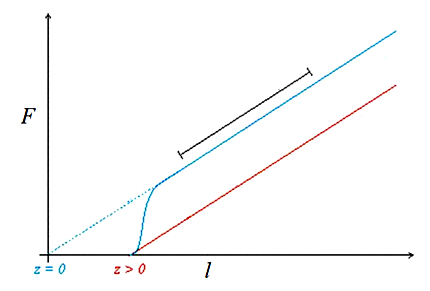
\includegraphics[width =1\linewidth]{15}
		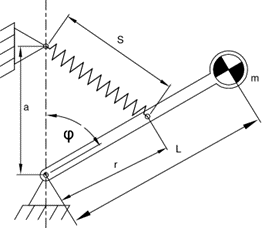
\includegraphics[width =1\linewidth]{15b}
		\caption{\small\textit{\color{timhieukhoahoc}Hình $13$. Trên: Sự phụ thuộc của lực đàn hồi vào độ dài lò xo của lò xo độ dài zero (xanh) và lò xo thông thường (đỏ). Dưới: một thiết bị đo trong lực theo dạng LaCoste, trong đó trọng lực tác dụng lên vật $m$ và lực đàn hồi của lò xo có cân bằng về momen quay.}}
		\vspace*{-10pt}
	\end{figure}
	Với các khảo sát bằng máy bay, do phải xử lý các gia tốc gây ra do lực quán tính khi máy bay chuyển động trên bầu trời, người ta thiết kế những thiết bị rất phức tạp gồm nhiều thành phần tương tự với các thiết bị đo momen xoắn từ thời Eötvös. Đồng thời, với sự ra đời của máy tính điện tử, bản đồ trọng lực có thể được thiết lập từ việc tính toán các dịch chuyển nhỏ của quỹ đạo các vệ tinh quay quanh Trái Đất. Đây cũng là một trong những công nghệ có vai trò quan trọng để tăng độ chính xác của việc định vị GPS.
	\vskip 0.1cm
	$\pmb{5.}$ \textbf{\color{timhieukhoahoc}Lời kết}
	\vskip 0.1cm
	Có thể thấy, trong khoa học và kỹ thuật, những vấn đề lý thuyết và thực nghiệm luôn đan xen thúc đẩy lẫn nhau. Những thí nghiệm cơ học của Galileo cũng như các kết quả thiên văn của Kepler lại cần đến giải tích của Newton để xây dựng lý thuyết về lực hấp dẫn. Đồng thời, trong khi Newton cho rằng người ta không thể nào đo lực hấp dẫn giữa các vật thể nhỏ hơn các thiên thể trong vũ trụ thì các nhà thực nghiệm lại chứng minh điều ngược lại nếu ta có thể thiết kế và sáng tạo được các dụng cụ và phương pháp đo đủ chính xác. Pi sẽ còn tiếp tục giới thiệu tới độc giả nhiều vấn đề thú vị khác trong lịch sử khoa học trong những số tiếp theo.
	\vskip 0.1cm
	\PIbox{Gần đây, một bài hát đã được sáng tác kể về thí nghiệm cân Trái Đất của Maskelyne. Độc giả quan tâm có thể tìm trên Internet bài hát mang tên Schiehallion của ca sĩ Iona Lane.}
	\vskip 0.1cm
	\textbf{\color{timhieukhoahoc}Tài liệu tham khảo}
	\vskip 0.1cm
	[$1$] Ferreiro, L. D. ($2011$). \textit{Measure of the Earth}. Basic Books.
	\vskip 0.1cm
	[$2$] Milsom, J. ($2018$). \textit{The Hunt for Earth Gravity : A History of Gravity Measurement from Galileo to the $21$st Century}. Springer International Publishing.
	\vskip 0.1cm
	[$3$] Smallwood, J. R. ($2007$). Maskelyne's $1774$ Schiehallion experiment revisited. \textit{Scottish Journal of Geology}, $43(1)$, $15-31$. \url{https://doi.org/10.1144/sjg43010015}
\end{multicols}


